\documentclass{article}

\usepackage{../../common/labconfig}
\usepackage{../../common/labstyle}

\lhead{Virtual SPI Lab (Multi-Slave)}

\begin{document}

\section{Introduction}

The objective of this lab will be to read streaming data from the VD-002
sensor, and to store it in the VD-003 flash memory device in a prescribed
format.

\begin{figure}[H]

	\centering

	\begin{tabular}{r|l}

		Part & Due Date \\ \hline\hline
		Code & Apr. 14\\

	\end{tabular}

	\caption{Table of due dates for each part.}

\end{figure}

\tableofcontents

\section{How to Submit }

When your code is ready to turn in, please submit only your \texttt{main.cpp}
file via Moodle. Note that you should write all code that you need within
\texttt{main.cpp}. As before, your code must compile to receive any credit.

\section{Simulated Devices}

In this lab, you will interface with two virtual devices using SPI, a sensor
and a flash memory.

\begin{figure}[H]

	\centering

        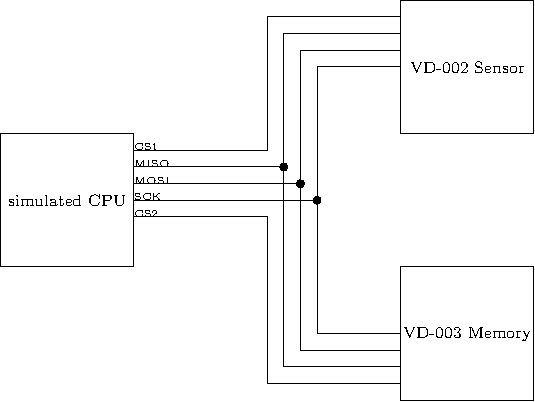
\includegraphics[max width = 0.7\textwidth]{topology.pdf}

	\caption{Topology of the simulated devices.}

\end{figure}


\subsection{VD-002: Simulated Sensor}

\textbf{Read this section carefully as it has changed since the previous lab.}

The VD-002 operates in two possible modes, depending on which register is
accessed. In \textbf{single} mode, the SPI master transmits a single 1-byte
register address, and the VD-002 will respond with a single 1-byte value
corresponding to that register's data. In \textbf{streaming} mode, the SPI
master transmits a single 1-byte register address, and the VD-002 will respond
with one or more bytes of data, sent continually within the same SPI
transaction. While operating in \textbf{streaming} mode, the SPI master device
must keep the chip select line held low and the clock driven continually.

\textbf{Unlike the sensor from the previous lab}, the VD-002 collects sensor
readings that may contain between 1 and 128 bytes of data. The \textbf{single}
mode works identically to the SPI transactions used to communicate with the
sensor in the previous lab, however the \textbf{streaming} mode is new, and
will require your code to be modified.

\begin{figure}[H]

	\centering

	\begin{tabular}{c | c | c | p{0.5\textwidth}}

		Register Address & Name & Mode & Description \\ \hline\hline

		\texttt{0x0F} & \texttt{WHO\_AM\_I} & single & Always contains the value \texttt{0x35} \\ \hline

		\texttt{0x10} & \texttt{DATA} & streaming & Returns a stream of 1 to 128 sensor readings. \\ \hline

		\texttt{0x11} & \texttt{DATACNT} & single & Returns the number of data values that would be streamed out if \texttt{DATA} is read. \\

	\end{tabular}

	\caption{Table of VD-002 registers.}

\end{figure}

To safely read the stream of data collected by the sensor, an application must
first read the \texttt{DATACNT} register. If this register returns a value of
0, then \texttt{DATA} cannot be read yet, and attempting to read it will result
in undefined behavior. Otherwise, the value read from \texttt{DATACNT} will
specify how many bytes the application should prepare to stream in from the
sensor.

If the chip-select is de-asserted (pulled high) or the clock is not driven
while the sensor is still streaming data out, then any remaining data in the
stream will be lost.

Note that once \texttt{DATACNT} is set to a non-zero value, the data ready to
stream out will not change until \texttt{DATA} is read.

\subsection{VD-003: Simulated Flash Memory}

The VD-003 simulates a flash memory storage device. This device operates in two
modes.  \textbf{Single} mode operates similarly to the \textbf{single} mode
described previously for the VD-002, with the additional requirement that the
most significant bit of the register address must be 0. In \textbf{write} mode,
the most significant bit of the register address should be 1. In \textbf{write}
mode, the SPI master transmits two bytes in order, and the VD-003 will keep the
MISO line held low. The first byte in \textbf{write} mode corresponds to the
register address, and the second byte corresponds to the value which is to be
written to that register.

To further clarify: the VD-003 utilizes 7-bit register addresses with a 1-bit
read/write flag, while the VD-002 utilizes 8-bit register addresses (since the
VD-002 has no writable registers).

\begin{figure}[H]

	\centering

	\begin{tabular}{c | c | c | p{0.5\textwidth}}

		Register Address & Name & Mode(s) & Description \\ \hline\hline

		\texttt{0x01} & \texttt{NPAGE} & single & Returns the number of pages on the flash device. \\ \hline

		\texttt{0x0F} & \texttt{WHO\_AM\_I} & single & Always contains the value \texttt{0x36} \\ \hline

		\texttt{0x10} & \texttt{PAGESEL} & single/write & Selects which page of memory is active. \\ \hline

		\texttt{0x11} & \texttt{OFFSET} & single/write & Determines the offset of the active byte relative to the beginning of the page. \\ \hline

		\texttt{0x12} & \texttt{DATA} & single/write & Specifies the value at the active address on the active page. \\


	\end{tabular}

	\caption{Table of VD-003 registers.}

\end{figure}

The VD-003 consists of between 1 and 256 pages of 256 bytes each. The "active
byte" may be read or written by performing either a read or write operation on
the \texttt{DATA} register. Which byte is "active" may be changed by modifying
the \texttt{PAGESEL} and \texttt{OFFSET} registers.

\subsection{Program Requirements}

Your program should first query the \texttt{WHO\_AM\_I} register and verify it
returns the correct value. If not, then your program should display an error
message (on standard out) and exit.

Your program should also query the \texttt{NPAGE} register of the VD-003 to
determine the number of pages of memory available.

Finally, your program should enter an infinite loop, polling the
\texttt{DATACNT} register of the VD-002 until data is ready, then streaming
that data into memory and writing it back out into the flash memory on the next
lowest data page which has not been used yet. Only one stream from reading the
\texttt{DATA} register should be stored per page in the VD-003.

The pages stored in the VD-003 flash memory should adhere to the following
format:

\begin{figure}[H]

	\centering

	\begin{tabular}{c | p{0.5\textwidth} }

		Offset & Description \\ \hline\hline

		\texttt{0x00} & A "magic number" \texttt{0x11} to signify that
		this page contains sensor data. \\ \hline

		\texttt{0x01} & The sequence number of this sensor reading. The
		first sensor reading read from the VD-002 should have a
		sequence number of 0. The next sensor reading should have a
		sequence number of 1. The one after that a sequence number of
		2, and so on. \\ \hline

		\texttt{0x02} & The number of data values $n$ in the sensor reading. \\ \hline

		\texttt{0x03} & The first data value in the sensor reading. \\ \hline

		$\dots$ & $\dots$ \\ \hline

		\texttt{0x03} + $n$ & The $n$th data value in the sensor reading. \\ \hline

		$\dots$ & All remaining bytes may contain any value (you do not need to update them). \\

	\end{tabular}

	\caption{Table describing required VD-003 page format.}

\end{figure}

Once your program has exhausted the available supply of flash memory pages (the
number of pages available can be determined by the \texttt{NPAGE} register of
the VD-003), it should exit with an informative message indicating no further
flash memory is available.

\section{Programming Environment}

The programming environment for this lab will be similar to the previous lab,
with the following notable changes:

\begin{itemize}

	\item The \texttt{IO\_CS} pin has been removed.

	\item The \texttt{IO\_CS1} pin has been added.

	\item The \texttt{IO\_CS2} pin has been added.

	\item A new \texttt{Makefile} target has been added: \texttt{make
		flashdump} which will display the contents of the flash memory
		based \texttt{trace.vcd}.

	\item The \texttt{refdump.txt} file contains the output of \texttt{make
		flashdump} from the reference solution after being run against
		the version of the sensor an flash memory provided in the
		project skeleton (i.e. if your code is correct, you should get
		the same output from \texttt{make flashdump}). Hint: this means
		it also contains the expected hard-coded sensor values.

\end{itemize}

\section{Suggested Plan of Work}

You may approach this lab in whatever manner you see fit. However, this section
provides a suggested list of tasks for you to tackle, in an order we think will
make it easiest for you.

\begin{itemize}

	\item Update your existing SPI driver code to allow specifying which
		chip select pin to use.

	\item Implement checks for the \texttt{WHO\_AM\_I} register using
		updated driver code.

	\item Read the value of \texttt{NPAGE} from the VD-003 and store it for
		later use.

	\item Implement a new function to support the streaming mode for the
		VD-002. One way\footnote{You could also use a linked list if
		you wish to implement one. Using C++'s \texttt{std::vector} is
		also allowed.} to handle the variable length of the sensor
		readings would be to \texttt{malloc()} an array of
		\texttt{DATACNT} + 1 many \texttt{uint8\_t} elements, using the
		first element to define the length of the array, and the
		remaining elements to store the sensor readings. Your function
		could return a pointer to this array. Your function should
		poll \texttt{DATACNT} until it returns a nonzero value.

	\item Be able to print out the streamed sensor readings.

	\item Implement a new function to support the VD-003's write mode. You
		can test if it is working by using \texttt{make flashdump}.

	\item Implement a new function which takes a 256-byte long array of
		\texttt{uint8\_t} values and writes it to a specified page on
		the VD-003.

	\item Implement a new function which reads in a stream of sensor data,
		generates an appropriately formatted page of data, then writes
		it using the function from the above bullet point.

	\item Call the function from the above bullet point in a loop until all
		pages are exhausted. You can use a simple counter to keep track
		of how many pages you are using and compare it against the read
		value of\texttt{NPAGE}.

\end{itemize}

Here are some \textbf{hints} you might find helpful while completing this lab:

\begin{itemize}

	\item The sequence number at offset \texttt{0x01} in the VD-003 page
		format will also be the page number, incidentally since pages
		are numbered starting at 0, and one page is used per sensor
		reading.

	\item You are allowed to use global variables to store the page
		counter, and/or the sensor data stream if you see fit. Remember
		you will never be streamed more than 128 bytes of data, so a
		global array of that size might be the easiest way to make this
		data available across functions.

	\item The value $n$ at offset \texttt{0x02} in the VD-003 page format
		will be the same value you read from \texttt{DATACNT} before
		streaming in the sensor data.

	\item You should use the values \texttt{CPOL}=1 and \texttt{CPHA}=1 for
		both devices.

	\item It is a good idea to define constants corresponding to all the
		important registers and offsets mentioned previously.

	\item This lab may look intimidating compared to the previous one,
		however if you completed the last lab successfully, this one
		should be a straightforward modification of your SPI driver
		code plus some glue logic. Don't over-think things!

\end{itemize}

\section{Grading}

Your code will be inspected for style and correctness by a human reader. This
aspect of grading will be fairly lenient and mostly for the purpose of giving
you useful feedback. However you may still lose points for egregious stylistic
problems, or failing to write code that clearly attempts to solve the problem
at hand.

Your code will also be run against the same simulated sensor as you are given
in the project skeleton, however the hard-coded sensor "readings" will be
changed to different values. \textbf{The length of sensor data streams and the
number of flash memory pages will also be changed during grading, so make sure
your program accounts for this.}

Additionally, your code will be run against a version of the simulated sensor
and/or flash memory which is defective, and reports an incorrect value when the
\texttt{WHO\_AM\_I} register is read. In such cases, your program should exit
with an informative error message. \textbf{You may assume that if a VD-002 or
VD-003 reports a correct \texttt{WHO\_AM\_I} value, it is not defective.}

The correctness of your code will primarily judged by evaluating the output of
\texttt{make flashdump} using an alternate set of sensor data, however any
printouts your code displays, as well as the output of sigrok via \texttt{make
decode} may be used as a supplement.

If your code does not compile and run on the CSCE linux lab computers, you will
not receive credit.

\section{Rubric}

\begin{itemize}

	\item 10 points - Code style

	\item 10 points - Correct checking of \texttt{WHO\_AM\_I} register

	\item 10 points - Data is requested and streamed from the sensor.

	\item 10 points - Data is stored in the VD-003 in the proper format.

	\item 10 points - Data stored in the VD-003 is correct/matches the
		hard-coded values from the sensor (format must also be
		correct).

	\item $\frac{5}{2} \times b$ points - See "Bug Bounty".


\end{itemize}

\textbf{Maximum number of points possible: 50.}

Keep in mind that some items not listed on the rubric may cause you to loose
points, including cheating, submitting code which is inconsistent with what you
have demonstrating, plagiarizing code or reflection content, etc.

\section{Bug Bounty (Extra Credit Opportunity)}

There is an extra credit opportunity available for this lab. If you find a bug
in our code, we will increment the $b$ counter in the rubric above once for
each bug. In other words, you will earn 2.5 bonus points per bug. If this puts
your grade on this project higher than 50 points, you will receive $b$ many
bonus points on the final exam (i.e. each bug you find will improve your final
exam score by 1\%).

To take advantage of this opportunity, you must send us an email with the
following example:

\begin{itemize}

	\item A zipped up copy of your code.

	\item A clear description of the bug and how to re-produce it.

	\item A clear description of how the bug causes the code to behave in a
		manner inconsistent with what is documented in this lab sheet,
		or in a fashion that is otherwise problematic.

\end{itemize}

If your bug stems from your own code, or a mis-understanding of the course
material, you will neither gain nor lose points ($b$ remains unchanged).
However submitting a bug report without all three of the items above will
result in $b$ being decremented, and possibly becoming negative as a result.

Minor typos, compiler warnings, etc. do not count as bugs, but please feel
welcome to report them if you find them.

If multiple students discover the same bug, they will all receive the bonus.
However, reports emailed after a fix has been announced or otherwise
distributed to the class are not eligible to receive the extra credit. To
receive the bonus, your bug report must be submitted no later than Monday,
April 27, 2020 at midnight eastern time.

\section*{Appendix I: Test Data Format}

\textbf{Note:} You do not need to read this section to complete the lab.

If you wish to test your code with alternate data besides what is provided, the
\texttt{sensordata.hex} file can be modified (this is how you will be graded).
This file contains the hard-coded "sensor" readings as ascii-encoded
hexadecimal values, one value per line. It may contain at most 8192 values,
which are organized as sensor data streams. Each stream begins with it's
length, followed by it's contents. After the final stream should be placed a
single line containing the value \texttt{0}, which signifies to the sensor
"hardware" that it should wrap back to the beginning of the file.

As an example, consider this \texttt{sensordata.hex}, which you may recognize
as containing the first two reading provided for this lab:

\begin{verbatim}
01
01
05
00
01
02
03
04
00
\end{verbatim}

This file would instruct the VD-002 hardware that the first stream is of length
1, and contains the value \texttt{0x01}. The second stream read would be of
length 5, and contains the values 0, 1, 2, 3, 4 in that order. The sensor would
then wrap back to the first stream (hence the first and third streams will have
the exact same content).

The script \texttt{makeranddata.py} was used to generate most of the data
streams in the provided \texttt{sensordata.hex} file. You are welcome to use it
to generate additional data streams if you feel so inclined.

If you choose to generate your own data streams for testing, you should keep a
backup of \texttt{sensordata.hex} so you can validate your flash dump with the
reference one provided.

\end{document}
